\documentclass[lecture_notes.tex]{subfiles}

\begin{document}

\notestitle{Session 2}{Exact Diagonalization of the Heisenberg Spin Chain}%
  {quantum\_magnetism.ipynb}{Session 1 (second quantization and the superexchange derivation of the
  Heisenberg model)}

\subsection*{Contents and goals}
In the last session we saw that mean-field theory has a limitation, since it only uses product
states and the ground state of the Hubbard dimer is a singlet, which is an entangled state that
does not break any symmetry. In this session we will not do any approximation. We will take the
Heisenberg Hamiltonian that we obtained from superexchange, write it as a matrix in the full
many-body Hilbert space, which has dimension $2^L$, and diagonalize it exactly. With this, we will
learn how to read a many-body spectrum. First, we will use the many-body gap to see if a spin chain
is gapped or gapless. Then we will see how a magnetic field or a change in the couplings gives rise
to level crossings and phase transitions. We will also see how symmetries allow us to write the
Hamiltonian in blocks, so that we can solve bigger systems, and how static and dynamical correlators
tell us about the order and the excitations of the system. At the end we will ask if the
excitations of a quantum magnet can be described as single-particle excitations, in terms of
emergent fermions that are called spinons. All the results in this session are exact, and the price
we pay is that the Hilbert space grows as $2^L$. This exponential growth is the reason why, starting
in Session 4, we will use tensor-network methods.

\subsection*{Learning outcomes}
By the end of this session, you should be able to do the following.
\begin{itemize}[nosep]
  \item Build the Heisenberg Hamiltonian as an explicit matrix in the basis of many-body product
    states and diagonalize it exactly for a finite spin chain.
  \item Use the finite-size scaling of the many-body gap, which either follows a power law or
    saturates, to tell a gapless spin chain from a gapped one.
  \item Use conserved quantum numbers, which are the total spin and $S_{\mathrm{tot}}^z$, to
    block-diagonalize the Hamiltonian, and explain level crossings and magnetization curves in a
    field.
  \item Compute static and dynamical spin correlators and connect them to a mean-field description
    of the excitations in terms of auxiliary fermions, which are called spinons.
\end{itemize}

\subsection{From the Hubbard dimer to a quantum magnet}
\label{sec:setup}
\subsubsection{The classical Ising dimer}
Let us start by recalling what a classical magnet with a broken symmetry looks like at the
microscopic level, since it is the natural contrast to what comes next. Let us take the simplest
magnetic Hamiltonian, which is an Ising coupling between two spins,
\begin{equation}
  \Ham_{\mathrm{Ising}} = J\, S_1^z S_2^z, \qquad J>0.
  \label{eq:isingdimer}
\end{equation}
There is no $S^x$ or $S^y$ in it, so we can think of $S_i^z=\pm\tfrac12$ as a classical Ising
variable. Minimizing the energy is simple, since we want $S_1^z$ and $S_2^z$ to have opposite sign,
and there are exactly two ways to do that, $\ket{\up\dn}$ and $\ket{\dn\up}$. Both are valid ground
states and both break time-reversal symmetry, because flipping every spin takes one into the other.
Each of them has a finite and well-defined local moment $\expval{S_i^z}=\pm\tfrac12$. This is a
small version of a classical magnet, which is a symmetry-broken state with a finite magnetization at
every site.

\subsubsection{The quantum Heisenberg dimer}
Now let us keep the full quantum mechanics of the spin operators and couple all three components,
\begin{equation}
  \Ham_{\mathrm{Heis}} = J\, \vb S_1\cdot\vb S_2 = J\left(S_1^xS_2^x + S_1^yS_2^y + S_1^zS_2^z\right).
  \label{eq:heisdimer}
\end{equation}
This is the superexchange Hamiltonian that we derived in the last session from the strong-coupling
limit of the Hubbard dimer, with $J=4t^2/U>0$. We already know from Session 1 that its exact ground
state is the singlet $\ket{\Psi_{\mathrm{singlet}}}=\tfrac{1}{\sqrt2}(\ket{\up\dn}-\ket{\dn\up})$,
which is a single non-degenerate state with $\expval{S_i^z}=0$ on every site, and which cannot be
written as a product state. From now on we will call this a \textbf{quantum magnet}. In
contrast with the Ising ground states, this state does not break time-reversal symmetry, and it is
entangled in an essential way. In this session we will compute this kind of ground state exactly,
for chains longer than two sites, and we will see what we can learn from it and from the excited
states above it.

\subsection{Exact diagonalization of a spin chain}
\label{sec:ed}
\subsubsection{The product-state basis}
Let us now generalize Eq.~\eqref{eq:heisdimer} to a chain of $L$ spin-$\tfrac12$'s with
nearest-neighbor exchange,
\begin{equation}
  \Ham_{\mathrm{Heis}} = J\sum_{i=1}^{L-1} \vb S_i\cdot\vb S_{i+1}, \qquad J>0
  \ \text{(antiferromagnetic).}
  \label{eq:heisenberg}
\end{equation}
Regardless of how complicated $J_{ij}$ is on a given lattice, solving this Hamiltonian exactly always
takes the same three steps. First we pick a basis of the many-body Hilbert space, then we write
$\Ham$ as a matrix in that basis, and finally we diagonalize it. The natural basis is the set of all
product states $\ket{\sigma_1\sigma_2\cdots\sigma_L}$ with $\sigma_i\in\{\up,\dn\}$. There are two
states for $L=1$, four for $L=2$, eight for $L=3$, and in general $2^L$ states for $L$ sites. This is
the same exponential growth of the many-body Hilbert space that we saw in Session 1 for the Hubbard
model. It appears here again because a spin-$\tfrac12$ chain is a projected part of that same
fermionic Hilbert space, where every site is singly occupied.

\subsubsection{A sparse matrix}
To build the matrix we need the matrix elements of $\vb S_i\cdot\vb S_j$, and it is convenient to
split it into a diagonal and an off-diagonal part using the raising and lowering operators
$S^\pm = S^x\pm iS^y$,
\begin{equation}
  \vb S_i\cdot\vb S_j = S_i^zS_j^z + \tfrac12\left(S_i^+S_j^- + S_i^-S_j^+\right).
  \label{eq:sdots}
\end{equation}
The first term is diagonal in our product basis, since it multiplies each basis state by
$\pm\tfrac14$ depending on whether $\sigma_i,\sigma_j$ are parallel or antiparallel. The second term
is the one that moves us inside the basis. The operator $S_i^+S_j^-$ flips an antiparallel pair
$\dn_i\up_j\to\up_i\dn_j$ and gives zero on everything else, so it only connects basis states that
differ by swapping one $\up\dn$ pair on two sites joined by a bond. This is why the Heisenberg
matrix is \emph{sparse}, even though it lives in a $2^L$-dimensional space, meaning that each row
has at most $L-1$ off-diagonal entries, one per bond. Iterative solvers such as Lanczos use this
structure to reach much bigger $L$ than a dense diagonalization can.
Figure~\ref{fig:ed-recipe} goes through the three steps for $L=4$.

\begin{figure}[H]
  \centering
  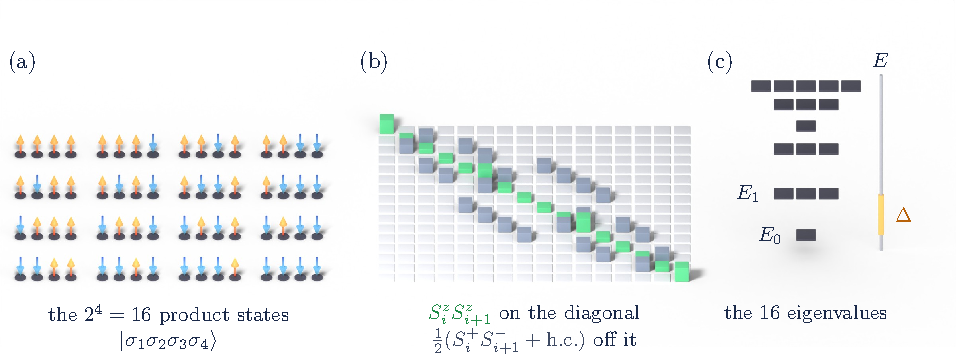
\includegraphics[width=\textwidth]{figures/quantum_magnetism/ed_recipe.pdf}
  \caption{The three steps of exact diagonalization for the open Heisenberg chain of
    Eq.~\eqref{eq:heisenberg} with $L=4$. (a) The basis, which is the $2^4=16$ product states in
    the order a code would count them, with $\ket{\up\up\up\up}$ at the back left and
    $\ket{\dn\dn\dn\dn}$ at the front right. (b) The Hamiltonian in that basis, with one cell per
    matrix element in the same order and the height of a bar giving the size of the element. The
    $S^z_iS^z_{i+1}$ term of Eq.~\eqref{eq:sdots} fills the diagonal and the flip-flop term puts at
    most $L-1=3$ bars in each row, so only $40$ of the $256$ cells are occupied, which is what we
    mean by a sparse matrix. (c) The result, which is the sixteen eigenvalues drawn as levels at
    their energy, with degenerate levels side by side. There is a singlet ground state at
    $E_0\approx-1.62J$, a triplet at $E_1\approx-0.96J$, and the many-body gap $\Delta=E_1-E_0$ of
    Eq.~\eqref{eq:manybodygap} in amber. At the top are the five members of the fully polarized
    $S=2$ multiplet at $\tfrac34J$.}
  \label{fig:ed-recipe}
\end{figure}

\subsubsection{The dimer solved in two ways}
Let us see this explicitly for $L=2$. In
the basis $\{\ket{\up\up},\ket{\up\dn},\ket{\dn\up},\ket{\dn\dn}\}$, the stretched states
$\ket{\up\up}$ and $\ket{\dn\dn}$ have no partner to flip into, so
$\Ham_{\mathrm{Heis}}\ket{\up\up}=\tfrac{J}{4}\ket{\up\up}$, and the same holds for $\ket{\dn\dn}$.
On the remaining two-dimensional subspace $\{\ket{\up\dn},\ket{\dn\up}\}$, Eq.~\eqref{eq:sdots}
gives the $2\times2$ block
\begin{equation}
  \Ham_{\mathrm{Heis}}\Big|_{\{\up\dn,\dn\up\}} = J\begin{pmatrix} -\tfrac14 & \tfrac12 \\[2pt]
    \tfrac12 & -\tfrac14 \end{pmatrix}
  \;\Longrightarrow\;
  E_\pm = J\left(-\tfrac14\pm\tfrac12\right), \qquad
  \ket{\pm} = \tfrac{1}{\sqrt2}\left(\ket{\up\dn}\pm\ket{\dn\up}\right).
  \label{eq:dimermatrix}
\end{equation}
So $E_-=-\tfrac34 J$ for the antisymmetric combination, which is the singlet we already knew, and
$E_+=\tfrac14 J$ for the symmetric combination, which is degenerate with $\ket{\up\up}$ and
$\ket{\dn\dn}$ at the same energy $\tfrac{J}{4}$. Together these three states form the
\textbf{triplet}. Diagonalizing a $4\times4$ matrix by hand already gives the full structure of the
singlet and the triplet.

There is a second and faster way to get the same answer, and we will use it again because it
generalizes. We define the total spin $\vb S_{\mathrm{tot}} = \vb S_1+\vb S_2$, so that
$\vb S_{\mathrm{tot}}^2 = \vb S_1^2+\vb S_2^2+2\,\vb S_1\cdot\vb S_2$, and hence
\begin{equation}
  \Ham_{\mathrm{Heis}} = J\,\vb S_1\cdot\vb S_2
    = \frac{J}{2}\left[S_{\mathrm{tot}}(S_{\mathrm{tot}}+1) - \tfrac34 - \tfrac34\right],
  \label{eq:dimerspec}
\end{equation}
where we used $\vb S_i^2=\tfrac34$ for spin-$\tfrac12$. Since $\vb S_{\mathrm{tot}}^2$ has
eigenvalues $S_{\mathrm{tot}}(S_{\mathrm{tot}}+1)$ with $S_{\mathrm{tot}}=0$ or $1$ for two
spin-$\tfrac12$'s, Eq.~\eqref{eq:dimerspec} directly gives $E(S_{\mathrm{tot}}=0)=-\tfrac34J$ and
$E(S_{\mathrm{tot}}=1)=\tfrac14J$, in exact agreement with Eq.~\eqref{eq:dimermatrix}. Note also why
the ground-state energy in the notebook is equal to the sum of the Ising and XY ground energies
computed separately. On the two-dimensional subspace $\{\ket{\up\dn},\ket{\dn\up}\}$, the Ising part
$S_1^zS_2^z$ is proportional to the identity, $-\tfrac14\mathbb{1}$, because \emph{both} basis states
have the same $S_1^zS_2^z$ eigenvalue. Minimizing the sum of a constant and the XY block is the same
as minimizing each one separately and adding them, and this is why the two energies add up here.
This only happens for $L=2$. For longer chains the Ising term is no longer a multiple of the identity
on the subspace that the XY term mixes, and in general the two parts no longer have their minimum on
the same state.

\begin{notebook}
Open \texttt{quantum\_magnetism.ipynb} and work through the ``Basics'' block, which has the sections
``Creating a spin\_chain object,'' ``Creating a Hamiltonian,'' ``Computing the ground state
energy,'' and ``Computing expectation values.'' Build the $L=2$ Heisenberg Hamiltonian directly from
the spin operators, diagonalize it, and check numerically that you get
$E_{\mathrm{singlet}}=-\tfrac34J$ and $E_{\mathrm{triplet}}=\tfrac14J$. Then replace $S^x$ by $S^y$
in the expectation-value cell and think about why nothing changes.
\end{notebook}

\subsection{The many-body spectrum and the many-body gap}
\label{sec:gap}
\subsubsection{Counting the eigenvalues}
Now let us leave the case $L=2$, which we can do by hand, and let the computer diagonalize
Eq.~\eqref{eq:heisenberg} for increasing $L$. The number of eigenvalues we obtain is the dimension of
the matrix, $2^L$, which is four for $L=2$, sixteen for $L=4$, sixty-four for $L=6$, and so on, so it
grows exponentially with system size in the same way as the basis. In practice, however, we almost
never need the whole spectrum. A real experiment at low temperature only probes the states closest
to the ground state, so from now on we will focus on the bottom of the many-body spectrum, which is
the ground state $E_0$ and the few low-lying excited states above it.

\subsubsection{The many-body gap and its scaling}
The most useful number that we can read from this part of the spectrum is the \textbf{many-body
gap},
\begin{equation}
  \Delta(L) \equiv E_1(L) - E_0(L),
  \label{eq:manybodygap}
\end{equation}
which is the energy cost of the lowest excitation above the ground state, and it is marked for $L=4$
in panel (c) of Figure~\ref{fig:ed-recipe}. For the uniform Heisenberg chain, $\Delta(L)$ decreases
steadily as $L$ grows, and it follows a power law instead of saturating to a finite value. This is
the signature of a \textbf{gapless} system, meaning that its excitations cost arbitrarily little
energy in the thermodynamic limit. Where does this power law come from? Qualitatively, it comes from
the same free-fermion argument that we will use in Section~\ref{sec:spinon}. If we replace each spin
operator by an auxiliary fermion $f_{i\sigma}$, which is called an Abrikosov fermion, and decouple
the exchange term at the mean-field level, $\Ham_{\mathrm{Heis}}$ becomes a free-fermion
\textbf{spinon} Hamiltonian with a gapless band and Fermi points at $k_F=\pm\pi/2$. The lowest
excitations are then particle-hole pairs created at those Fermi points, which disperse
\emph{linearly} in momentum. A linearly dispersing excitation on a ring of $L$ sites is a
one-dimensional particle-in-a-box problem, so its levels are spaced by
\begin{equation}
  \Delta(L) \;\sim\; \frac{\pi v_s}{L},
  \label{eq:gapscaling}
\end{equation}
with $v_s$ the velocity of the low-energy excitations, meaning that the gap follows a $1/L$ power law
and does not stay finite. Numerically, the finite-size data is well described by
$\Delta(L)\approx\pi^2J/(2L)$. To obtain $v_s$ with this precision we need the exact Bethe-ansatz
solution, since mean-field theory gives the right qualitative power law but not the precise
coefficient. We will keep this picture of a particle in a box in mind, because we will see it again
in a more literal form when we look at dynamical correlators in Section~\ref{sec:dynamical}, and
again when we build the explicit spinon band structure behind this argument in
Section~\ref{sec:spinon}.

\begin{notebook}
Section ``Many-body energies of the Heisenberg model.'' Diagonalize the uniform chain for
$L=2,4,6,8$ and plot the full spectrum each time, and check that the number of eigenvalues is
$2^L$. Then plot only $E_1(L)-E_0(L)$ and see how the gap shrinks with $L$. Think also about the
biggest $L$ for which you could still store the full spectrum on your own machine.
\end{notebook}

\subsection{The XXZ model from classical order to entanglement}
\label{sec:xxz}
\subsubsection{The two ends of the XXZ chain}
Section~\ref{sec:setup} presented the Ising model and the Heisenberg model as two separate
Hamiltonians, but it is more useful to see them as the two ends of a single family. Let us take
\begin{equation}
  \Ham_{\mathrm{XXZ}} = \sum_i \left[J_{xy}\left(S_i^xS_{i+1}^x + S_i^yS_{i+1}^y\right)
    + J_z\, S_i^zS_{i+1}^z\right], \qquad J_z\equiv 1 \text{ fixed},
  \label{eq:xxz}
\end{equation}
and change $J_{xy}$ from $0$ to $1$. At $J_{xy}=0$ we are back at the classical Ising model of
Eq.~\eqref{eq:isingdimer}, generalized to $L$ sites. In the thermodynamic limit its ground state is
doubly degenerate, with the N\'eel-ordered state $\ket{\up\dn\up\dn\cdots}$ and its time-reversed
partner, and each of them has a finite staggered moment that breaks the symmetry. At $J_{xy}=1$ we
recover the isotropic Heisenberg model of Eq.~\eqref{eq:heisenberg}, whose ground state, as we
already know from the dimer, is unique and has no local moment, so it is a purely quantum magnet.
This means that $J_{xy}$ interpolates between a classical magnet with a broken symmetry and an
entangled quantum magnet, and the natural question is how the ground state goes from one description
to the other as we change $J_{xy}$.

\begin{figure}[H]
  \centering
  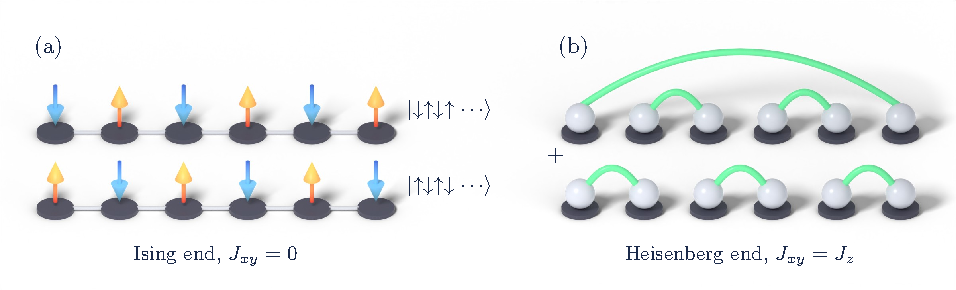
\includegraphics[width=\textwidth]{figures/quantum_magnetism/neel_pair.pdf}
  \caption{The two ends of Eq.~\eqref{eq:xxz}. (a) The two classical ground states at the Ising
    end $J_{xy}=0$, with $\ket{\up\dn\up\dn\cdots}$ in front and $\ket{\dn\up\dn\up\cdots}$ behind
    it. Each is a product state with a definite $S^z$ on every site, each has a finite staggered
    moment, and the two are exchanged by time reversal. In the thermodynamic limit they are exactly
    degenerate and the system picks one of them, which is what symmetry breaking means here. On a
    finite chain, once $J_{xy}$ is switched on, they are instead split by a tiny amount, and the
    growth of this splitting as $J_{xy}\to1$ is how the crossover to the unique, entangled
    Heisenberg ground state appears in the spectrum. (b) At the Heisenberg end $J_{xy}=J_z$ there is
    no moment on any site, so the spins are drawn as spheres without arrows. You can think of the
    ground state as neighbors paired into singlets, drawn as the green bonds, which resonate between
    the two ways of pairing them. The two pairings are drawn in front and behind, and the second one
    pairs the two ends as on a ring. This is a cartoon of the entanglement and not the exact state,
    which also contains singlets between distant sites.}
  \label{fig:neel-pair}
\end{figure}

\subsubsection{The transition in the finite-size spectrum}
The finite-size spectrum answers this question directly. At small $J_{xy}$ the two classical N\'eel
states are not exactly degenerate on a finite chain, since only an infinite chain can spontaneously
break a symmetry. However, they are very close in energy, and we can see the tiny splitting between
them directly on the screen, which is what remains of the classical double degeneracy at finite
size. As we increase $J_{xy}$ toward $1$, this splitting grows continuously, and for any finite $L$
it becomes a finite gap between two clearly non-degenerate states once $J_{xy}$ is close enough to
$1$. What changes as we make $L$ bigger is how close to $J_{xy}=1$ this crossover is. For longer
chains, the two low-lying states stay nearly degenerate over a longer range of $J_{xy}$, and the
crossover becomes sharper and approaches the exact transition of the XXZ chain in the thermodynamic
limit, which the Bethe-ansatz solution places exactly at the isotropic, SU(2)-symmetric point
$J_{xy}=J_z$. In other words, just by following how two eigenvalues of a finite-size spectrum move
and split as we change a coupling constant, we can already detect a quantum phase transition, before
we reach the thermodynamic limit. We will use this technique many times in the rest of the course.

\begin{notebook}
Section ``From classical to quantum magnetism.'' Plot the low-lying spectrum of
$\Ham_{\mathrm{XXZ}}$ as a function of $J_{xy}$ at fixed $L$. Identify the near-degenerate pair at
small $J_{xy}$ and follow how it splits as $J_{xy}\to1$. Then increase $L$ and see how the crossover
of the splitting becomes sharper and moves, following the exact transition of the thermodynamic
limit at the isotropic point.
\end{notebook}

\subsection{Good quantum numbers of the Heisenberg chain}
\label{sec:quantumnumbers}
\subsubsection{Conservation of the total spin}
Section~\ref{sec:ed} used the identity $\vb S_1\cdot\vb S_2=\tfrac12[\vb S_{\mathrm{tot}}^2 - \vb
S_1^2-\vb S_2^2]$ as a shortcut for the dimer, and it is useful to ask why it worked. The reason is
that $\vb S_{\mathrm{tot}}^2$ and $S_{\mathrm{tot}}^z$ commute with $\Ham_{\mathrm{Heis}}$, and this
is not special to two sites. Because Eq.~\eqref{eq:heisenberg} is built only from dot products
$\vb S_i\cdot\vb S_j$, it is invariant under any global spin rotation. Noether's theorem in its
operator form then tells us that the total spin $\vb S_{\mathrm{tot}}=\sum_i \vb S_i$ is conserved
for \emph{any} $L$ and any choice of exchange couplings $J_{ij}$, which we write as
\begin{equation}
  \left[\Ham_{\mathrm{Heis}},\, \vb S_{\mathrm{tot}}^2\right] = 0, \qquad
  \left[\Ham_{\mathrm{Heis}},\, S_{\mathrm{tot}}^z\right] = 0.
  \label{eq:conservation}
\end{equation}
So every eigenstate of $\Ham_{\mathrm{Heis}}$ can be labeled by a definite total spin $S$ and a
definite projection $m$. These are the singlet ($S=0$) and triplet ($S=1$) labels that we used for
the dimer, which now become good quantum numbers for a chain of any length.

\subsubsection{The Zeeman field does not mix states}
Let us now add a uniform magnetic field,
\begin{equation}
  \Ham(B) = \Ham_{\mathrm{Heis}} - B\, S_{\mathrm{tot}}^z.
  \label{eq:zeeman}
\end{equation}
This term singles out the $z$-axis, so it breaks the full SU(2) spin-rotation symmetry down to
rotations about $z$ only. However, let us look at what it does to our two conserved quantities. It
commutes with $S_{\mathrm{tot}}^z$, since it is built only from this operator. And because
$[\vb S_{\mathrm{tot}}^2, S_{\mathrm{tot}}^z]=0$ is a general identity of the algebra of angular
momentum, $\Ham(B)$ \emph{also} commutes with $\vb S_{\mathrm{tot}}^2$. So both quantum numbers
survive in the presence of the field, meaning that adding $B$ cannot mix eigenstates of
$\Ham_{\mathrm{Heis}}$ with each other, and it can only shift the energy of each one by $-Bm$. This
is why the spectrum as a function of the field that you see in the notebook is a set of straight
lines and not of curves. Each state with a definite $m$ shifts linearly, $E(B)=E(0)-Bm$, and states
only bend or avoid each other once we add a term that does not commute with $S_{\mathrm{tot}}^z$,
such as a transverse field.

Let us apply this to the dimer. The singlet has $m=0$ and stays flat, $E_{\mathrm{singlet}}(B)=-\tfrac34
J$. The three members of the triplet split according to their own $m=-1,0,+1$. The $m=0$ member is
also flat, at $E=\tfrac14J$, while the $m=\pm1$ members disperse as $E=\tfrac14J\mp B$. These are the
two flat lines that you can see in the zero-field spectrum of the notebook. They are at different
energies, separated by exactly the many-body gap $\Delta=J$ of Eq.~\eqref{eq:manybodygap}, and what
distinguishes them is not $m$, which is $0$ for both, but the total spin $S$, which is $0$ for one
and $1$ for the other.

\subsubsection{Block-diagonalizing a long chain}
The main use of Eq.~\eqref{eq:conservation} is
computational. Since $S_{\mathrm{tot}}^z=\sum_i S_i^z$ is conserved, the full $2^L\times2^L$
Hamiltonian never mixes basis states with different numbers of up spins. If $n_\up$ counts the up
spins, then $m=n_\up-L/2$ is fixed within each block, and $\Ham_{\mathrm{Heis}}$ is block-diagonal
with blocks of dimension
\begin{equation}
  \dim(m) = \binom{L}{L/2+m}.
  \label{eq:szsector}
\end{equation}
The largest block is at $m=0$ (for even $L$), with $\dim(0)=\binom{L}{L/2}\sim 2^L/\sqrt{\pi L/2}$
from Stirling's approximation. This is still exponential in $L$, but it is a factor $\sim\sqrt L$
smaller than the full Hilbert space, and what matters most is that it can be diagonalized
independently of every other block. If the chain is also periodic, translational invariance gives us
a second conserved quantity, which is the total momentum $k$, and combining $S_{\mathrm{tot}}^z$
sectors with momentum sectors makes the largest block smaller by roughly another factor of $L$.
Using every available conserved quantity together with the sparse-matrix Lanczos techniques of
Section~\ref{sec:ed} is how exact-diagonalization codes reach the $L\sim20$ spins that are the limit
of this session. Without it, $2^{20}\approx10^6$ would already be a heavy dense-matrix computation,
and $L=30$ would be out of reach.

\begin{figure}[H]
  \centering
  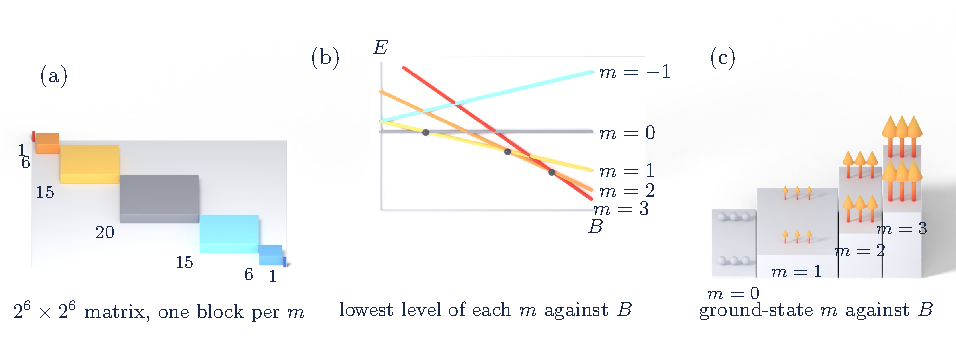
\includegraphics[width=\textwidth]{figures/quantum_magnetism/sz_blocks.pdf}
  \caption{What the conservation of $S_{\mathrm{tot}}^z$ gives us, for the open chain of $L=6$.
    (a) Block structure of $\Ham_{\mathrm{Heis}}$ in the $S_{\mathrm{tot}}^z$ basis, with the blocks
    to scale and $m=+3$ at the back. Because $S_{\mathrm{tot}}^z$ is conserved, the Hamiltonian
    never connects basis states with different numbers of up spins, so the $2^L\times2^L$ matrix
    splits into one block per magnetization sector, of dimension $\binom{L}{L/2+m}$ as in
    Eq.~\eqref{eq:szsector}, and every element outside the blocks is zero. Each block is
    diagonalized independently of the others, and even the largest one, at $m=0$, is already
    smaller than the full space by a factor $\sim\sqrt L$. (b) The lowest level of each block, in
    the color of its block, as a function of the field of Eq.~\eqref{eq:zeeman}. We leave out $m=-2$
    and $m=-3$, which rise out of the frame immediately. Every line is straight,
    $E_m(B)=E_m(0)-Bm$, and the dark beads mark where a different block takes over the bottom of
    the fan, at $B\approx0.49J$, $1.39J$ and $1.87J$. (c) The ground-state magnetization obtained
    from (b), which is the staircase of Section~\ref{sec:levelcrossings}, with the chain standing on
    each plateau. On the singlet plateau the spins are spheres with no moment, and on the next
    plateaus they are arrows whose length is the average moment $m/L$ per site. The moment is
    saturated from $B=J[1+\cos(\pi/L)]\approx1.87J$ on, which is the one-magnon edge of the open
    chain and tends to the $2J$ of the infinite chain as $L$ grows.}
  \label{fig:sz-blocks}
\end{figure}

\begin{notebook}
Sections ``Energies of a Heisenberg model as a function of the external magnetic field'' and
``Quantum numbers in the Heisenberg model.'' Plot the dimer spectrum as a function of $B$ and check
the linear evolution without mixing that Eq.~\eqref{eq:zeeman} predicts. Identify which line is the
singlet and which is the $m=0$ member of the triplet, and check that they are exactly $\Delta=J$
apart at $B=0$. Then think about which field-dependent term would bend the lines instead of keeping
them straight.
\end{notebook}

\subsection{Level crossings and magnetization curves}
\label{sec:levelcrossings}
\subsubsection{The level crossing of the dimer}
Equation~\eqref{eq:zeeman} does more than split levels. Since different $m$-sectors disperse with
different slopes, they can cross, and a crossing at the bottom of the spectrum is a
\textbf{level crossing of the ground state}. For the dimer we can find it exactly. The ground state
is the singlet, at $-\tfrac34J$, until the $m=+1$ triplet branch $E=\tfrac14J-B$ goes below it,
which happens when
\begin{equation}
  \tfrac14J - B = -\tfrac34J \quad\Longrightarrow\quad B = J.
  \label{eq:crossingfield}
\end{equation}
Below $B=J$ the ground state is the singlet, with zero magnetization, and above $B=J$ it is the fully
polarized member of the triplet $\ket{\up\up}$, with saturated magnetization
$\expval{S_{\mathrm{tot}}^z}=1$. This is the simplest example of a quantum phase transition driven by
a field, which here is a single sharp level crossing between a sector with $S=0$ and a sector with
$S=1$.

\subsubsection{The magnetization staircase of longer chains}
Longer chains show the same phenomenon, repeated many times. As $B$ grows from zero, the ground state
moves step by step through sectors of increasing total spin, $S=0\to1\to2\to3\to\cdots$, and each
step appears as a sudden jump in the ground-state magnetization $\expval{S_{\mathrm{tot}}^z}$, which
gives a magnetization staircase. Panels (b) and (c) of Figure~\ref{fig:sz-blocks} show both for
$L=6$, the crossings at the bottom of the fan and the staircase that they give. Because bigger
chains have their low-lying $S$-sectors closer together in energy, these crossings happen at smaller
and smaller fields as $L$ grows, and in the thermodynamic limit the staircase becomes the continuous
magnetization curve of an infinite antiferromagnetic chain. Once $B$ is larger than roughly the
bandwidth of the low-energy spectrum, which is $B\gtrsim zJ$ with $z$ the coordination number, the
ground state saturates completely and every spin points along the field. For a chain, $z=2$ and the
saturation field is exactly $B_{\mathrm{sat}}=2J$. This fully polarized state is in fact an
\emph{exact} eigenstate of $\Ham_{\mathrm{Heis}}$ itself, and it is a rare case where the many-body
ground state is a simple product state, since the exchange term has nothing left to do once every
spin is maximally aligned. Changing $B\to-B$ gives the same staircase with the opposite sign of
magnetization, which is the time-reversal partner of the $B>0$ curve.

\subsubsection{Excited states in a small field}
Let us also look at the excited states in a small field, before any level crossing has happened. The
ground state stays a total-$S=0$ singlet with zero magnetization on every site. The first excited
states, which are the $S=1$ members of the triplet, do have a finite total magnetization, but this
magnetization is not localized anywhere. Instead, it is spread over the whole chain, which is one
more sign that these are delocalized many-body excitations and not a single flipped spin at one
site. Higher excited states repeat this pattern with different sign structures, and several of them
are related to each other by time reversal. This whole family of spread-out excitations, which look
roughly like the states of a particle in a box, is what the dynamical correlator of
Section~\ref{sec:dynamical} will allow us to resolve in detail.

\begin{notebook}
Sections ``Level crossings in the Heisenberg model,'' ``Many-body wavefunctions in a magnetic
field,'' ``Level crossings as a function of the magnetic field,'' and ``Magnetization of moderately
large Heisenberg model.'' Check the crossing of the dimer at $B=J$ from Eq.~\eqref{eq:crossingfield}.
Then move to chains with $L=6$ and $L=10$ and follow the full magnetization staircase, its
saturation field, and its mirror symmetry under $B\to-B$.
\end{notebook}

\subsection{The gapped dimerized chain}
\label{sec:dimerization}
\subsubsection{A chain with alternating bonds}
Section~\ref{sec:gap} told us that the uniform Heisenberg chain is gapless, with $\Delta(L)\to0$ as a
power law. Let us now build a chain that is gapped, by alternating the exchange coupling from bond to
bond,
\begin{equation}
  \Ham_{\mathrm{dimer}} = \sum_i J_i\, \vb S_i\cdot\vb S_{i+1}, \qquad
  J_i = J\left[1+(-1)^i\delta\right],
  \label{eq:dimerized}
\end{equation}
so odd and even bonds alternate between $J(1+\delta)$ and $J(1-\delta)$. At $\delta=0$ we recover the
uniform, gapless chain. At the opposite limit $\delta\to1$, the weak bonds vanish and the chain
splits into $L/2$ decoupled dimers, each one exactly the $L=2$ problem of Section~\ref{sec:ed}. The
exact ground state is then a product of singlets, one per strong bond, and the lowest excitation is a
single dimer going from its singlet into its triplet, which costs exactly
$\Delta_\infty = J(1+\delta)$, the same singlet-triplet gap that we computed in
Eq.~\eqref{eq:dimermatrix}. Turning the weak bond back on changes this picture, since the singlets
now couple to each other and the triplet excitation gets some dispersion, but it does not close the
gap. For any finite $\delta$, no matter how small, the dimerized chain stays gapped, with a finite
$\Delta_\infty$ that goes smoothly to zero only as $\delta\to0$.
Figure~\ref{fig:dimerized} shows the two chains side by side.

\begin{figure}[H]
  \centering
  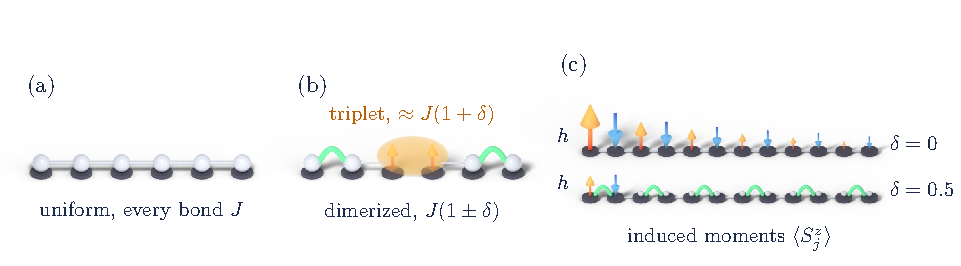
\includegraphics[width=\textwidth]{figures/quantum_magnetism/dimerized.pdf}
  \caption{The uniform and the dimerized chain of Eq.~\eqref{eq:dimerized}. (a) At $\delta=0$
    every bond is the same and no pair of sites is singled out. (b) At finite $\delta$ the strong
    bonds, drawn as green singlets, alternate with weak ones, drawn thin. The lowest excitation is
    one strong bond lifted from its singlet into a triplet, here its $m=+1$ member with both spins
    up, which costs about $J(1+\delta)$ and is what keeps the chain gapped. (c) A field $h$ pins the
    first spin of a chain of $L=12$, and the arrows are the induced moments $\expval{S_j^z}$ of the
    exact ground state, to scale, for $h=0.2J$. Along the uniform chain at the back they alternate
    in sign and decay slowly, which is the algebraic decay of Section~\ref{sec:diagnostics}, and
    since on the open chain they add up to zero, the far end compensates. Along the dimerized chain
    in front, with $\delta=0.5$ and its strong bonds drawn as singlets, the first singlet takes
    almost all of the response and the moment is gone by the third dimer, which is the exponential
    decay set by $\xi$. Moments below $0.02$ are drawn as small spheres.}
  \label{fig:dimerized}
\end{figure}

\subsubsection{Finite-size convergence of the gap}
This qualitative difference appears very clearly in how $\Delta(L)$ approaches its value in the
thermodynamic limit. For the gapless uniform chain, we already saw the slow power-law approach of
Eq.~\eqref{eq:gapscaling}, and even $L\sim20$ is not enough to be sure that the gap goes to zero. For the dimerized chain, a finite gap defines its own length scale, which is the correlation
length $\xi\sim v_s/\Delta_\infty$, and the finite-size corrections to the gap are suppressed
exponentially, $\Delta(L)-\Delta_\infty \sim e^{-L/\xi}$, and not as a power law. This is why,
numerically, the gap of a dimerized chain already looks converged at $L\sim12$ to $14$, while the
gap of the uniform chain still changes visibly at the same size. The presence or absence of a length
scale $\xi$ is what separates fast, exponential finite-size convergence from slow, power-law
convergence.

\begin{notebook}
Section ``Gap of a many-body spin chain.'' Compute $\Delta(L)$ for the uniform chain ($\delta=0$)
and for a dimerized chain ($\delta>0$), and compare how fast each one saturates as you increase
$L$. Check that the dimerized gap has converged well before the uniform one.
\end{notebook}

\subsection{Diagnosing the gap with impurities and correlators}
\label{sec:diagnostics}
Comparing gaps at different $L$ works, but it needs several system sizes. Is there a way to tell
gapped from gapless behavior with a \emph{single} calculation? There is, and the way we do this is by
looking at how the system responds in space, instead of how its energy changes with size.

\subsubsection{A magnetic impurity}
Let us put a small local field on one site, $\Ham\to\Ham_{\mathrm{Heis}} - h\,
S_{i_0}^z$, and measure the induced magnetization profile $\expval{S_j^z}$ as a function of the
distance $r=|j-i_0|$ from the impurity. For the gapless uniform chain, this response decays
\emph{algebraically}, $\expval{S_j^z}\sim r^{-1}$, which is the usual signature of critical,
scale-free correlations in a one-dimensional gapless system. For the gapped dimerized chain, the same
measurement decays \emph{exponentially}, $\expval{S_j^z}\sim e^{-r/\xi}$, with the same correlation
length $\xi$ that controlled the finite-size convergence of the gap in
Section~\ref{sec:dimerization}. Panel (c) of Figure~\ref{fig:dimerized} shows both profiles for a
chain of twelve sites. So the way the response to a local perturbation dies out as we move away from
it already tells us, from a single system size, if the chain is gapped or gapless.

\subsubsection{Non-local static correlators}
We can get the same information without any impurity, by
computing the connected two-point correlator
\begin{equation}
  C(i,j) = \expval{\vb S_i\cdot\vb S_j} - \expval{\vb S_i}\cdot\expval{\vb S_j}.
  \label{eq:correlator}
\end{equation}
In a quantum magnet $\expval{\vb S_i}=0$ everywhere, so this reduces to the bare correlator
$\expval{\vb S_i\cdot\vb S_j}$. For a classical magnet described by a product state, on the other
hand, $C(i,j)$ is exactly zero, since in a product state the expectation value factorizes. So a
nonzero $C(i,j)$ is a direct signature of entanglement beyond any mean-field description, which is
the same failure of mean-field theory that we found for the Hubbard dimer in Session 1. Formally,
this static correlator is related to the impurity response of the previous paragraph by linear
response, through a Kubo-formula argument, meaning that the magnetization induced at $j$ by a small
field at $i$ is, to leading order, proportional to $C(i,j)$ itself. As a result, $C(i,j)$ shows the
same two behaviors, with power-law decay for the gapless chain and exponential decay, with a rate set
by $\delta$, for the dimerized one. The bigger the dimerization, the bigger the gap and the faster
$C(i,j)$ decays, which gives a diagnostic from a single calculation for how gapped a quantum magnet
is.

\begin{notebook}
Sections ``Magnetization of a Heisenberg model with a magnetic impurity,'' ``Magnetization of a
dimerized Heisenberg model with a magnetic impurity,'' and ``Non-local static correlators.'' Compare
the decay of the induced magnetization for the uniform and the dimerized chains. Then compute
Eq.~\eqref{eq:correlator} directly for several values of the dimerization and check that a faster
decay goes together with a bigger gap.
\end{notebook}

\subsection{Dynamical correlators, and a first look at spin-1}
\label{sec:dynamical}
\subsubsection{The Lehmann representation}
So far we have only used static, equal-time expectation values. A \textbf{dynamical spin correlator}
contains more information, because it resolves excitations by their energy as well as by their
position. We define
\begin{equation}
  S(i,\omega) = \bra{0}S_i^z\,\delta(\omega - (\Ham-E_0))\,S_i^z\ket{0}.
  \label{eq:dyncorrdef}
\end{equation}
This looks abstract, but it becomes clearer once we insert a resolution of the identity in the exact
eigenbasis of $\Ham$, $\mathbb{1}=\sum_n\ket{n}\bra{n}$, which turns Eq.~\eqref{eq:dyncorrdef} into
the Lehmann representation
\begin{equation}
  S(i,\omega) = \sum_n \left|\bra{n}S_i^z\ket{0}\right|^2 \, \delta\!\left(\omega - (E_n-E_0)\right).
  \label{eq:lehmann}
\end{equation}
We can read this as a spectroscopy experiment. If we inject a spin flip at site $i$ with energy
$\omega$, we get a nonzero response exactly when there is an eigenstate $\ket{n}$ at energy
$E_n=E_0+\omega$ that is connected to the ground state by a local spin flip, and the weight is given
by the size of the overlap $\bra{n}S_i^z\ket{0}$.

\subsubsection{Discrete peaks of the uniform chain}
For the spin-$\tfrac12$ uniform chain, $S(i,\omega)$ shows a sequence of discrete peaks, spread over
the whole chain and separated by gaps, which is the particle-in-a-box quantization that we
anticipated in Eq.~\eqref{eq:gapscaling}. As $L$ grows, these peaks move to lower $\omega$, following
the shrinking many-body gap of Section~\ref{sec:gap}, and more of them appear as the low-energy
spectrum becomes denser.

\subsubsection{A first look at spin-1}
If we do the same calculation for a spin-$1$ Heisenberg chain
instead of spin-$\tfrac12$, the profile of $S(i,\omega)$ looks qualitatively different. The reason
for this is that the two cases are in different phases. The spin-$\tfrac12$ chain is gapless in the
thermodynamic limit, as we have seen in this session, while the spin-$1$ chain is what is called a
\textbf{topological quantum magnet}, which has a full gap in the bulk but gapless, fractionalized
spin-$\tfrac12$ excitations pinned to the two ends of an open chain. Half-integer and integer spin
chains behave so differently because of the Lieb--Schultz--Mattis theorem, which says that a
translationally invariant, SU(2)-symmetric chain with half-integer spin per site cannot have a
unique, gapped ground state, while it puts no such restriction on integer spin. In our small
finite-size dynamical correlators we can already see hints of this, in the form of a low-energy
excitation that lives mostly at the two edges and becomes softer as $L$ grows, well below a much
larger bulk gap that roughly does not depend on the size. To resolve this fractionalization clearly,
however, we need system sizes well beyond what exact diagonalization can reach, and this is the job
that tensor networks will do for us in Session 4.

\begin{notebook}
Section ``Dynamical correlators.'' Compute $S(i,\omega)$ for the spin-$\tfrac12$ Heisenberg chain,
make the system smaller and follow how the discrete peaks move. Then add a magnetic field to see how
the Zeeman shifts of Section~\ref{sec:quantumnumbers} appear directly in the peak positions of the
correlator.
\end{notebook}

\subsection{Spinon mean-field theory with Abrikosov fermions}
\label{sec:spinon}
\subsubsection{A single-particle picture of the excitations}
Everything we have computed so far treats the ground state and its excitations as many-body objects,
without any single-particle description. However, we can ask the same question that we asked in
Session 1 about the Hubbard model, which is whether there is an auxiliary single-particle Hamiltonian
whose spectrum reproduces, at least qualitatively, the low-energy excitations of
$\Ham_{\mathrm{Heis}}$. The answer is yes, and it comes from writing the quantum spin operators
themselves in terms of auxiliary fermions.

\subsubsection{The Abrikosov auxiliary fermion representation}
We introduce one fermion $f_{i\sigma}$
per site and per spin flavor and write
\begin{equation}
  S_i^\alpha = \frac12\sum_{\sigma\sigma'} f^\dagger_{i\sigma}\,\tau^\alpha_{\sigma\sigma'}\,f_{i\sigma'},
  \qquad \alpha=x,y,z,
  \label{eq:abrikosov}
\end{equation}
with $\tau^\alpha$ the Pauli matrices, together with the local constraint $\sum_\sigma
f^\dagger_{i\sigma}f_{i\sigma}=1$ on every site, meaning that there is exactly one auxiliary fermion
per site, no more and no fewer. This constraint is an essential part of the construction, since it
is what makes the representation exact and not approximate. A spinful fermion per site without the
constraint has four states, which are the empty state, the singly occupied states ($\up$ or $\dn$)
and the doubly occupied state. The constraint removes the empty and the doubly occupied
configurations and leaves exactly the two singly occupied states $\{\ket{\up},\ket{\dn}\}$, which is
the spin-$\tfrac12$ Hilbert space we started with. These auxiliary fermions are not electrons. They
never hop in or out of the constrained subspace, and they only describe the same two-dimensional
local Hilbert space in the language of fermions. Panel (a) of Figure~\ref{fig:abrikosov} shows the
four states of one site and the two that the constraint keeps.

\begin{figure}[H]
  \centering
  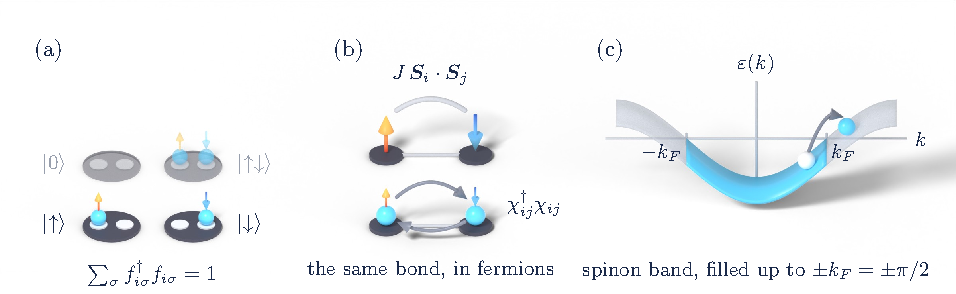
\includegraphics[width=\textwidth]{figures/quantum_magnetism/abrikosov.pdf}
  \caption{Spins as Abrikosov fermions, Eq.~\eqref{eq:abrikosov}. (a) One site as two fermion
    slots, $\up$ on the left and $\dn$ on the right, and its four states. The empty and the doubly
    occupied ones, drawn ghosted, are removed by the constraint, and the two that remain are exactly
    the spin-$\tfrac12$. (b) One bond drawn twice, with the spin exchange at the back and the same
    two sites in the language of fermions at the front. There Eq.~\eqref{eq:bondop} replaces the
    exchange by the bond operator, where the up fermion hops across the bond in one direction and
    the down fermion in the other direction, which leaves one fermion per site and the two spins
    flipped. (c) The spinon band $\varepsilon(k)=-J\chi\cos k$ of the uniform chain, from
    Eq.~\eqref{eq:mfspinon}, filled up to the Fermi points $k_F=\pm\pi/2$, with a particle-hole pair
    at the right Fermi point, made of a hole just below $k_F$ and a spinon just above it. This is the
    excitation that costs arbitrarily little energy, and it gives the gapless spinons behind
    Eq.~\eqref{eq:gapscaling}.}
  \label{fig:abrikosov}
\end{figure}

\subsubsection{Mean-field decoupling of the exchange}
Substituting Eq.~\eqref{eq:abrikosov} into $\vb S_i\cdot\vb S_j$ and using the constraint on each
site, one finds the identity
\begin{equation}
  \vb S_i\cdot\vb S_j = -\frac12\, \chi_{ij}^\dagger\chi_{ij} + \frac14 n_i n_j, \qquad
  \chi_{ij} \equiv \sum_\sigma f^\dagger_{i\sigma}f_{j\sigma},
  \label{eq:bondop}
\end{equation}
where $\chi_{ij}$ is the fermionic \textbf{bond operator}, shown in panel (b) of
Figure~\ref{fig:abrikosov}. This turns the quartic spin exchange into a quartic fermion interaction,
which is the kind of term that we learned to handle in Session 1, by decoupling it at the mean-field
level. We introduce the self-consistent bond amplitude
$\chi_{ij}\equiv\expval{\sum_\sigma f^\dagger_{i\sigma}f_{j\sigma}}$ and Lagrange multipliers
$\lambda_i$ that enforce the occupancy constraint on average, and Eq.~\eqref{eq:bondop} becomes an
effective free-fermion Hamiltonian, which is called the \textbf{spinon} Hamiltonian,
\begin{equation}
  \HMF = -\sum_{ij}\frac{J_{ij}\chi_{ij}}{2}\sum_\sigma f^\dagger_{i\sigma}f_{j\sigma} + \mathrm{h.c.}
    + \sum_i \lambda_i\left(n_i - 1\right).
  \label{eq:mfspinon}
\end{equation}
This is the same kind of self-consistency loop as in the Hubbard mean-field theory of Session 1. We
guess $\chi_{ij}$, diagonalize the resulting single-particle Hamiltonian, compute $\chi_{ij}$ again
from the filled spinon orbitals, and repeat until convergence.

\subsubsection{Spinon bands of the uniform and dimerized chains}
The advantage is that Eq.~\eqref{eq:mfspinon} is a tight-binding model, and we already know how to
read its spectrum. For the uniform chain, the self-consistent $\chi_{ij}\equiv\chi$ is the same on
every bond, which gives a simple cosine spinon band $\varepsilon(k) = -J\chi\cos k$ with gapless
Fermi points, and therefore gapless spin excitations, as shown in panel (c) of
Figure~\ref{fig:abrikosov}. This agrees with everything we found directly from exact diagonalization
in Section~\ref{sec:gap}. For the dimerized chain of Eq.~\eqref{eq:dimerized}, the bond amplitude
follows the alternation of $J_i$, which gives a dimerized tight-binding chain for the spinons,
similar to the Su-Schrieffer-Heeger model. Its spectrum opens a gap set by the difference between
the hopping amplitudes of the strong and the weak bonds, in the same way as the many-body gap of
Section~\ref{sec:dimerization}. The same construction can be generalized to two dimensions, where a
similar mean-field ansatz on, for example, the honeycomb lattice gives gapless \textbf{Dirac
spinons}, which is the auxiliary-fermion language behind many candidate quantum spin liquids. We
will not compute spinon bands in the notebook, but this picture is useful to keep, since it is the
language in which most proposals for quantum spin liquids are written.

\subsection*{Closing summary}
\begin{itemize}[nosep]
  \item Exact diagonalization means writing the Heisenberg Hamiltonian as a matrix in the full $2^L$
    product-state basis and diagonalizing it directly, without any restriction to product states.
    The exact singlet ($-\tfrac34J$) and triplet ($\tfrac14J$) energies of the dimer are the smallest
    worked example of this.
  \item The many-body gap $\Delta(L)=E_1-E_0$ shrinks with system size. A power-law decay signals a
    gapless chain, such as the uniform Heisenberg chain with $\Delta\sim\pi^2J/2L$, while saturation
    to a finite value, with exponentially fast finite-size convergence, signals a gapped chain, such
    as the dimerized chain.
  \item The XXZ model interpolates continuously between the classical, symmetry-broken Ising limit
    and the quantum, entangled Heisenberg limit. The finite-size splitting of the two lowest states
    already shows where the exact phase transition of the thermodynamic limit is.
  \item The total spin $\vb S_{\mathrm{tot}}^2$ and $S_{\mathrm{tot}}^z$ are exactly conserved
    quantities of the Heisenberg Hamiltonian, for any $L$. They block-diagonalize the exponentially
    large Hilbert space into much smaller sectors, they guarantee that a uniform field only splits
    levels linearly and does not mix them, and they are what allows exact diagonalization to reach
    $L\lesssim20$ spins.
  \item A sequence of level crossings driven by the field, between successive total-spin sectors,
    gives the magnetization staircase of a finite chain. Impurity responses and non-local static
    correlators decay algebraically when the chain is gapless and exponentially when it is gapped,
    so they diagnose from a single calculation the same physics as the gap scaling.
  \item Dynamical correlators resolve excitations in both space and energy through the Lehmann
    representation. Comparing spin-$\tfrac12$ and spin-$1$ chains gives our first hint of the
    fractionalized, topological physics of the spin-$1$ chain, which we will study properly with
    tensor networks in Session 4.
  \item Writing spins as constrained Abrikosov fermions and decoupling the exchange term at the
    mean-field level gives an effective free-fermion description of the excitations in terms of
    spinons. The spinons are gapless for the uniform chain and gapped for the dimerized chain, and
    the self-consistency loop is the same as in the Hubbard mean-field theory of Session 1.
  \item All of this is numerically exact, but the cost is still exponential in $L$. Even with every
    symmetry that we can use, exact diagonalization stops around $L\sim20$ spins, and this limit is
    the reason why we will use the matrix-product-state methods of Session 4.
\end{itemize}

\end{document}
